\documentclass[1p]{elsarticle_modified}
%\bibliographystyle{elsarticle-num}

%\usepackage[colorlinks]{hyperref}
%\usepackage{abbrmath_seonhwa} %\Abb, \Ascr, \Acal ,\Abf, \Afrak
\usepackage{amsfonts}
\usepackage{amssymb}
\usepackage{amsmath}
\usepackage{amsthm}
\usepackage{scalefnt}
\usepackage{amsbsy}
\usepackage{kotex}
\usepackage{caption}
\usepackage{subfig}
\usepackage{color}
\usepackage{graphicx}
\usepackage{xcolor} %% white, black, red, green, blue, cyan, magenta, yellow
\usepackage{float}
\usepackage{setspace}
\usepackage{hyperref}

\usepackage{tikz}
\usetikzlibrary{arrows}

\usepackage{multirow}
\usepackage{array} % fixed length table
\usepackage{hhline}

%%%%%%%%%%%%%%%%%%%%%
\makeatletter
\renewcommand*\env@matrix[1][\arraystretch]{%
	\edef\arraystretch{#1}%
	\hskip -\arraycolsep
	\let\@ifnextchar\new@ifnextchar
	\array{*\c@MaxMatrixCols c}}
\makeatother %https://tex.stackexchange.com/questions/14071/how-can-i-increase-the-line-spacing-in-a-matrix
%%%%%%%%%%%%%%%

\usepackage[normalem]{ulem}

\newcommand{\msout}[1]{\ifmmode\text{\sout{\ensuremath{#1}}}\else\sout{#1}\fi}
%SOURCE: \msout is \stkout macro in https://tex.stackexchange.com/questions/20609/strikeout-in-math-mode

\newcommand{\cancel}[1]{
	\ifmmode
	{\color{red}\msout{#1}}
	\else
	{\color{red}\sout{#1}}
	\fi
}

\newcommand{\add}[1]{
	{\color{blue}\uwave{#1}}
}

\newcommand{\replace}[2]{
	\ifmmode
	{\color{red}\msout{#1}}{\color{blue}\uwave{#2}}
	\else
	{\color{red}\sout{#1}}{\color{blue}\uwave{#2}}
	\fi
}

\newcommand{\Sol}{\mathcal{S}} %segment
\newcommand{\D}{D} %diagram
\newcommand{\A}{\mathcal{A}} %arc


%%%%%%%%%%%%%%%%%%%%%%%%%%%%%5 test

\def\sl{\operatorname{\textup{SL}}(2,\Cbb)}
\def\psl{\operatorname{\textup{PSL}}(2,\Cbb)}
\def\quan{\mkern 1mu \triangleright \mkern 1mu}

\theoremstyle{definition}
\newtheorem{thm}{Theorem}[section]
\newtheorem{prop}[thm]{Proposition}
\newtheorem{lem}[thm]{Lemma}
\newtheorem{ques}[thm]{Question}
\newtheorem{cor}[thm]{Corollary}
\newtheorem{defn}[thm]{Definition}
\newtheorem{exam}[thm]{Example}
\newtheorem{rmk}[thm]{Remark}
\newtheorem{alg}[thm]{Algorithm}

\newcommand{\I}{\sqrt{-1}}
\begin{document}

%\begin{frontmatter}
%
%\title{Boundary parabolic representations of knots up to 8 crossings}
%
%%% Group authors per affiliation:
%\author{Yunhi Cho} 
%\address{Department of Mathematics, University of Seoul, Seoul, Korea}
%\ead{yhcho@uos.ac.kr}
%
%
%\author{Seonhwa Kim} %\fnref{s_kim}}
%\address{Center for Geometry and Physics, Institute for Basic Science, Pohang, 37673, Korea}
%\ead{ryeona17@ibs.re.kr}
%
%\author{Hyuk Kim}
%\address{Department of Mathematical Sciences, Seoul National University, Seoul 08826, Korea}
%\ead{hyukkim@snu.ac.kr}
%
%\author{Seokbeom Yoon}
%\address{Department of Mathematical Sciences, Seoul National University, Seoul, 08826,  Korea}
%\ead{sbyoon15@snu.ac.kr}
%
%\begin{abstract}
%We find all boundary parabolic representation of knots up to 8 crossings.
%
%\end{abstract}
%\begin{keyword}
%    \MSC[2010] 57M25 
%\end{keyword}
%
%\end{frontmatter}

%\linenumbers
%\tableofcontents
%
\newcommand\colored[1]{\textcolor{white}{\rule[-0.35ex]{0.8em}{1.4ex}}\kern-0.8em\color{red} #1}%
%\newcommand\colored[1]{\textcolor{white}{ #1}\kern-2.17ex	\textcolor{white}{ #1}\kern-1.81ex	\textcolor{white}{ #1}\kern-2.15ex\color{red}#1	}

{\Large $\underline{12a_{0257}~(K12a_{0257})}$}

\setlength{\tabcolsep}{10pt}
\renewcommand{\arraystretch}{1.6}
\vspace{1cm}\begin{tabular}{m{100pt}>{\centering\arraybackslash}m{274pt}}
\multirow{5}{120pt}{
	\centering
	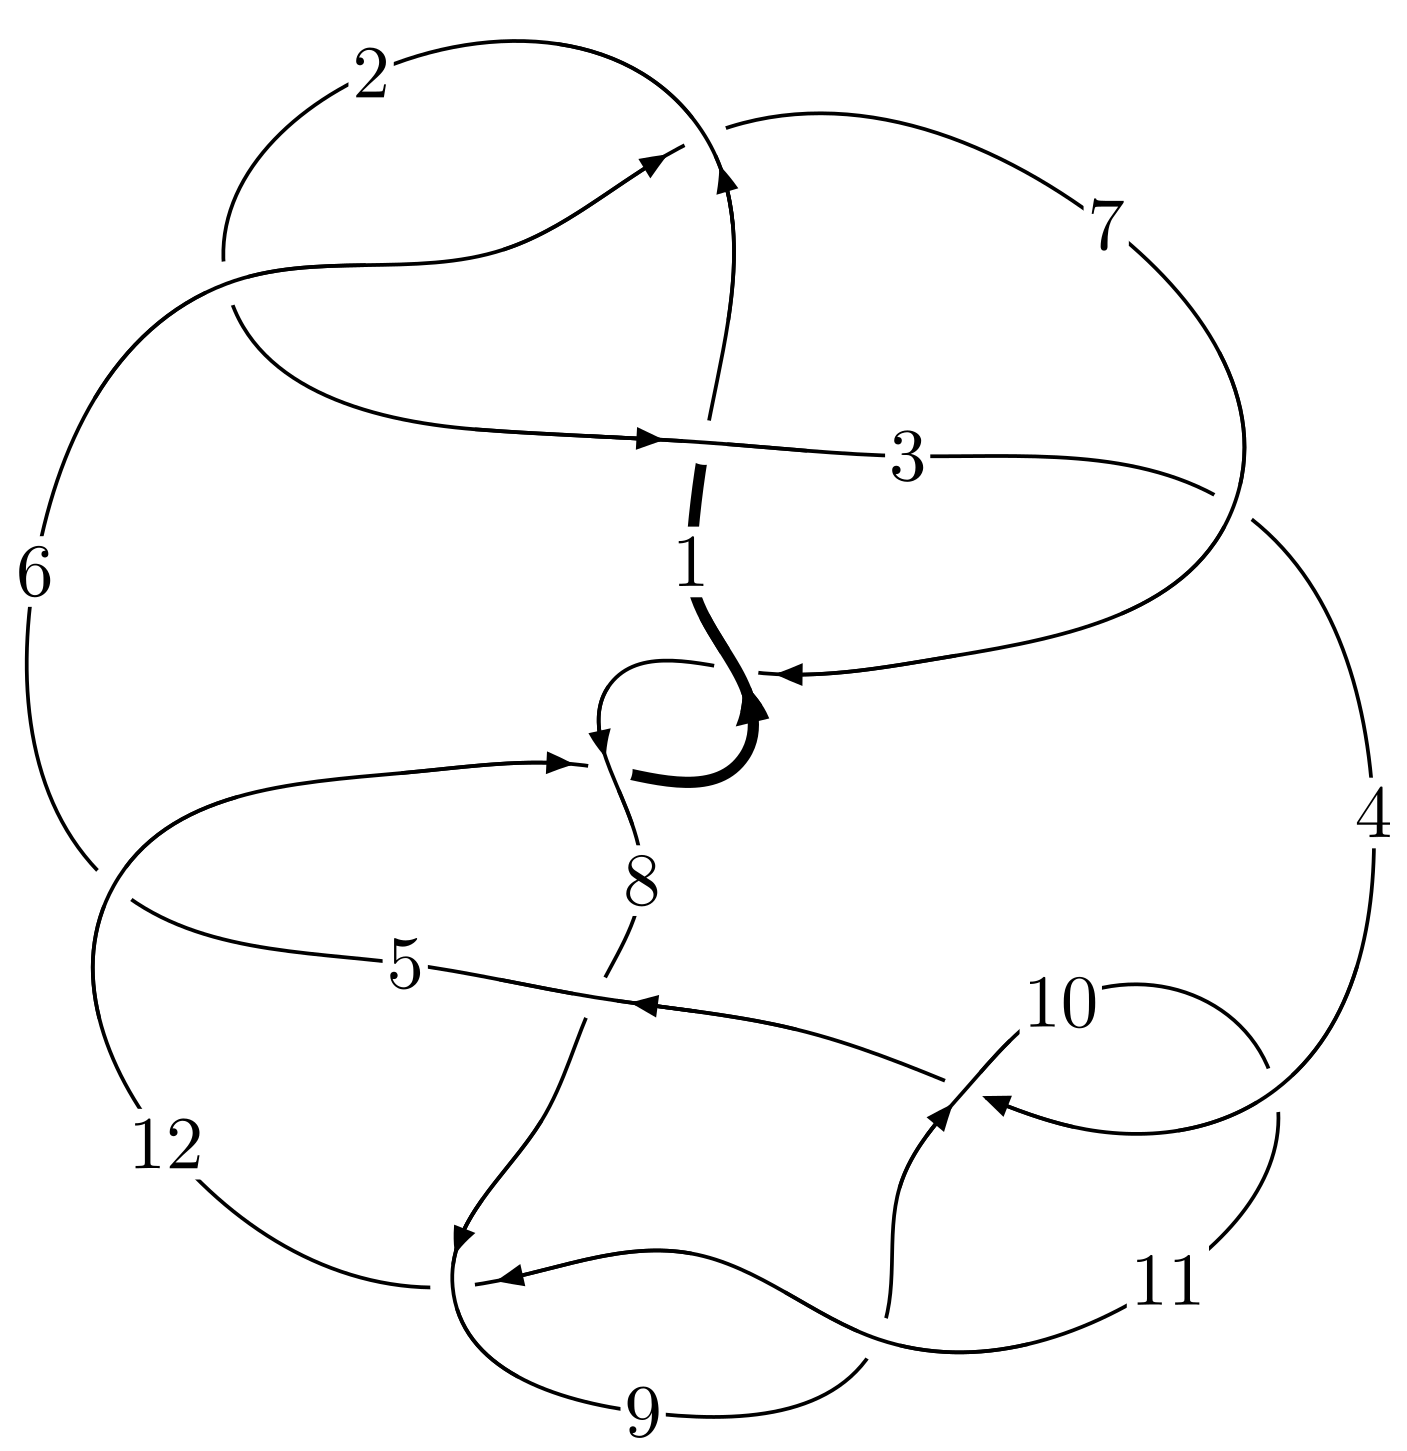
\includegraphics[width=112pt]{../../../GIT/diagram.site/Diagrams/png/1058_12a_0257.png}\\
\ \ \ A knot diagram\footnotemark}&
\allowdisplaybreaks
\textbf{Linearized knot diagam} \\
\cline{2-2}
 &
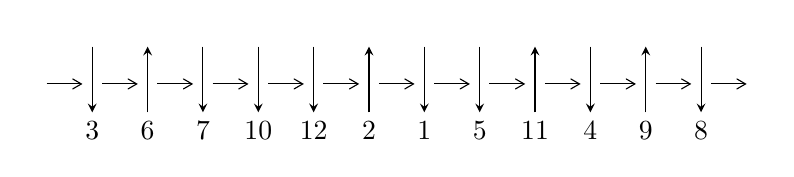
\begin{tikzpicture}[x=20pt, y=17pt]
	% nodes
	\node (C0) at (0, 0) {};
	\node (C1) at (1, 0) {};
	\node (C1U) at (1, +1) {};
	\node (C1D) at (1, -1) {3};

	\node (C2) at (2, 0) {};
	\node (C2U) at (2, +1) {};
	\node (C2D) at (2, -1) {6};

	\node (C3) at (3, 0) {};
	\node (C3U) at (3, +1) {};
	\node (C3D) at (3, -1) {7};

	\node (C4) at (4, 0) {};
	\node (C4U) at (4, +1) {};
	\node (C4D) at (4, -1) {10};

	\node (C5) at (5, 0) {};
	\node (C5U) at (5, +1) {};
	\node (C5D) at (5, -1) {12};

	\node (C6) at (6, 0) {};
	\node (C6U) at (6, +1) {};
	\node (C6D) at (6, -1) {2};

	\node (C7) at (7, 0) {};
	\node (C7U) at (7, +1) {};
	\node (C7D) at (7, -1) {1};

	\node (C8) at (8, 0) {};
	\node (C8U) at (8, +1) {};
	\node (C8D) at (8, -1) {5};

	\node (C9) at (9, 0) {};
	\node (C9U) at (9, +1) {};
	\node (C9D) at (9, -1) {11};

	\node (C10) at (10, 0) {};
	\node (C10U) at (10, +1) {};
	\node (C10D) at (10, -1) {4};

	\node (C11) at (11, 0) {};
	\node (C11U) at (11, +1) {};
	\node (C11D) at (11, -1) {9};

	\node (C12) at (12, 0) {};
	\node (C12U) at (12, +1) {};
	\node (C12D) at (12, -1) {8};
	\node (C13) at (13, 0) {};

	% arrows
	\draw[->,>={angle 60}]
	(C0) edge (C1) (C1) edge (C2) (C2) edge (C3) (C3) edge (C4) (C4) edge (C5) (C5) edge (C6) (C6) edge (C7) (C7) edge (C8) (C8) edge (C9) (C9) edge (C10) (C10) edge (C11) (C11) edge (C12) (C12) edge (C13) ;	\draw[->,>=stealth]
	(C1U) edge (C1D) (C2D) edge (C2U) (C3U) edge (C3D) (C4U) edge (C4D) (C5U) edge (C5D) (C6D) edge (C6U) (C7U) edge (C7D) (C8U) edge (C8D) (C9D) edge (C9U) (C10U) edge (C10D) (C11D) edge (C11U) (C12U) edge (C12D) ;
	\end{tikzpicture} \\
\hhline{~~} \\& 
\textbf{Solving Sequence} \\ \cline{2-2} 
 &
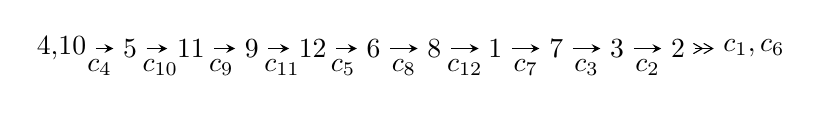
\begin{tikzpicture}[x=22pt, y=7pt]
	% node
	\node (A0) at (-1/8, 0) {4,10};
	\node (A1) at (1, 0) {5};
	\node (A2) at (2, 0) {11};
	\node (A3) at (3, 0) {9};
	\node (A4) at (4, 0) {12};
	\node (A5) at (5, 0) {6};
	\node (A6) at (6, 0) {8};
	\node (A7) at (7, 0) {1};
	\node (A8) at (8, 0) {7};
	\node (A9) at (9, 0) {3};
	\node (A10) at (10, 0) {2};
	\node (C1) at (1/2, -1) {$c_{4}$};
	\node (C2) at (3/2, -1) {$c_{10}$};
	\node (C3) at (5/2, -1) {$c_{9}$};
	\node (C4) at (7/2, -1) {$c_{11}$};
	\node (C5) at (9/2, -1) {$c_{5}$};
	\node (C6) at (11/2, -1) {$c_{8}$};
	\node (C7) at (13/2, -1) {$c_{12}$};
	\node (C8) at (15/2, -1) {$c_{7}$};
	\node (C9) at (17/2, -1) {$c_{3}$};
	\node (C10) at (19/2, -1) {$c_{2}$};
	\node (A11) at (45/4, 0) {$c_{1},c_{6}$};

	% edge
	\draw[->,>=stealth]	
	(A0) edge (A1) (A1) edge (A2) (A2) edge (A3) (A3) edge (A4) (A4) edge (A5) (A5) edge (A6) (A6) edge (A7) (A7) edge (A8) (A8) edge (A9) (A9) edge (A10) ;
	\draw[->>,>={angle 60}]	
	(A10) edge (A11);
\end{tikzpicture} \\ 

\end{tabular} \\

\footnotetext{
The image of knot diagram is generated by the software ``\textbf{Draw programme}" developed by Andrew Bartholomew(\url{http://www.layer8.co.uk/maths/draw/index.htm\#Running-draw}), where we modified some parts for our purpose(\url{https://github.com/CATsTAILs/LinksPainter}).
}\phantom \\ \newline 
\centering \textbf{Ideals for irreducible components\footnotemark of $X_{\text{par}}$} 
 
\begin{align*}
I^u_{1}&=\langle 
u^{95}- u^{94}+\cdots+2 u+1\rangle \\
\\
\end{align*}
\raggedright * 1 irreducible components of $\dim_{\mathbb{C}}=0$, with total 95 representations.\\
\footnotetext{All coefficients of polynomials are rational numbers. But the coefficients are sometimes approximated in decimal forms when there is not enough margin.}
\newpage
\renewcommand{\arraystretch}{1}
\centering \section*{I. $I^u_{1}= \langle u^{95}- u^{94}+\cdots+2 u+1 \rangle$}
\flushleft \textbf{(i) Arc colorings}\\
\begin{tabular}{m{7pt} m{180pt} m{7pt} m{180pt} }
\flushright $a_{4}=$&$\begin{pmatrix}1\\0\end{pmatrix}$ \\
\flushright $a_{10}=$&$\begin{pmatrix}0\\u\end{pmatrix}$ \\
\flushright $a_{5}=$&$\begin{pmatrix}1\\u^2\end{pmatrix}$ \\
\flushright $a_{11}=$&$\begin{pmatrix}- u\\u\end{pmatrix}$ \\
\flushright $a_{9}=$&$\begin{pmatrix}- u^3\\u^3+u\end{pmatrix}$ \\
\flushright $a_{12}=$&$\begin{pmatrix}- u^5- u\\u^5+u^3+u\end{pmatrix}$ \\
\flushright $a_{6}=$&$\begin{pmatrix}- u^{12}- u^{10}-3 u^8-2 u^6-2 u^4- u^2+1\\u^{12}+2 u^{10}+4 u^8+4 u^6+3 u^4+2 u^2\end{pmatrix}$ \\
\flushright $a_{8}=$&$\begin{pmatrix}u^5+u\\u^7+u^5+2 u^3+u\end{pmatrix}$ \\
\flushright $a_{1}=$&$\begin{pmatrix}- u^{17}-2 u^{15}-5 u^{13}-6 u^{11}-7 u^9-6 u^7-4 u^5-2 u^3- u\\- u^{19}-3 u^{17}-8 u^{15}-13 u^{13}-17 u^{11}-17 u^9-12 u^7-6 u^5- u^3+u\end{pmatrix}$ \\
\flushright $a_{7}=$&$\begin{pmatrix}u^{29}+4 u^{27}+\cdots+2 u^3+u\\u^{31}+5 u^{29}+\cdots+12 u^7+u\end{pmatrix}$ \\
\flushright $a_{3}=$&$\begin{pmatrix}- u^{60}-9 u^{58}+\cdots- u^2+1\\- u^{62}-10 u^{60}+\cdots-24 u^8- u^2\end{pmatrix}$ \\
\flushright $a_{2}=$&$\begin{pmatrix}u^{86}+13 u^{84}+\cdots+2 u^2+1\\- u^{86}-14 u^{84}+\cdots+6 u^4- u^2\end{pmatrix}$\\&\end{tabular}
\flushleft \textbf{(ii) Obstruction class $= -1$}\\~\\
\flushleft \textbf{(iii) Cusp Shapes $= 4 u^{93}-4 u^{92}+\cdots-12 u-10$}\\~\\
\newpage\renewcommand{\arraystretch}{1}
\flushleft \textbf{(iv) u-Polynomials at the component}\newline \\
\begin{tabular}{m{50pt}|m{274pt}}
Crossings & \hspace{64pt}u-Polynomials at each crossing \\
\hline $$\begin{aligned}c_{1}\end{aligned}$$&$\begin{aligned}
&u^{95}+43 u^{94}+\cdots+8 u^2-1
\end{aligned}$\\
\hline $$\begin{aligned}c_{2},c_{6}\end{aligned}$$&$\begin{aligned}
&u^{95}- u^{94}+\cdots-2 u+1
\end{aligned}$\\
\hline $$\begin{aligned}c_{3}\end{aligned}$$&$\begin{aligned}
&u^{95}+u^{94}+\cdots+14 u+1
\end{aligned}$\\
\hline $$\begin{aligned}c_{4},c_{10}\end{aligned}$$&$\begin{aligned}
&u^{95}- u^{94}+\cdots+2 u+1
\end{aligned}$\\
\hline $$\begin{aligned}c_{5}\end{aligned}$$&$\begin{aligned}
&u^{95}- u^{94}+\cdots-92 u+137
\end{aligned}$\\
\hline $$\begin{aligned}c_{7},c_{12}\end{aligned}$$&$\begin{aligned}
&u^{95}-5 u^{94}+\cdots-32 u+1
\end{aligned}$\\
\hline $$\begin{aligned}c_{8}\end{aligned}$$&$\begin{aligned}
&u^{95}+5 u^{94}+\cdots+294 u+133
\end{aligned}$\\
\hline $$\begin{aligned}c_{9},c_{11}\end{aligned}$$&$\begin{aligned}
&u^{95}-31 u^{94}+\cdots+48 u^3+1
\end{aligned}$\\
\hline
\end{tabular}\\~\\
\newpage\renewcommand{\arraystretch}{1}
\flushleft \textbf{(v) Riley Polynomials at the component}\newline \\
\begin{tabular}{m{50pt}|m{274pt}}
Crossings & \hspace{64pt}Riley Polynomials at each crossing \\
\hline $$\begin{aligned}c_{1}\end{aligned}$$&$\begin{aligned}
&y^{95}+19 y^{94}+\cdots+16 y-1
\end{aligned}$\\
\hline $$\begin{aligned}c_{2},c_{6}\end{aligned}$$&$\begin{aligned}
&y^{95}+43 y^{94}+\cdots+8 y^2-1
\end{aligned}$\\
\hline $$\begin{aligned}c_{3}\end{aligned}$$&$\begin{aligned}
&y^{95}-5 y^{94}+\cdots+128 y-1
\end{aligned}$\\
\hline $$\begin{aligned}c_{4},c_{10}\end{aligned}$$&$\begin{aligned}
&y^{95}+31 y^{94}+\cdots+48 y^3-1
\end{aligned}$\\
\hline $$\begin{aligned}c_{5}\end{aligned}$$&$\begin{aligned}
&y^{95}-9 y^{94}+\cdots+896772 y-18769
\end{aligned}$\\
\hline $$\begin{aligned}c_{7},c_{12}\end{aligned}$$&$\begin{aligned}
&y^{95}+71 y^{94}+\cdots-160 y-1
\end{aligned}$\\
\hline $$\begin{aligned}c_{8}\end{aligned}$$&$\begin{aligned}
&y^{95}+11 y^{94}+\cdots-932876 y-17689
\end{aligned}$\\
\hline $$\begin{aligned}c_{9},c_{11}\end{aligned}$$&$\begin{aligned}
&y^{95}+67 y^{94}+\cdots+240 y^2-1
\end{aligned}$\\
\hline
\end{tabular}\\~\\
\newpage\flushleft \textbf{(vi) Complex Volumes and Cusp Shapes}
$$\begin{array}{c|c|c}  
\text{Solutions to }I^u_{1}& \I (\text{vol} + \sqrt{-1}CS) & \text{Cusp shape}\\
 \hline 
\begin{aligned}
u &= -0.025374 + 0.996365 I\end{aligned}
 & \phantom{-}3.39359 + 2.05855 I & \phantom{-0.000000 } 0 \\ \hline\begin{aligned}
u &= -0.025374 - 0.996365 I\end{aligned}
 & \phantom{-}3.39359 - 2.05855 I & \phantom{-0.000000 } 0 \\ \hline\begin{aligned}
u &= \phantom{-}0.688552 + 0.710603 I\end{aligned}
 & -1.61555 + 2.05010 I & \phantom{-0.000000 } 0 \\ \hline\begin{aligned}
u &= \phantom{-}0.688552 - 0.710603 I\end{aligned}
 & -1.61555 - 2.05010 I & \phantom{-0.000000 } 0 \\ \hline\begin{aligned}
u &= \phantom{-}0.162735 + 0.962083 I\end{aligned}
 & -0.62221 - 5.79334 I & \phantom{-0.000000 } 0 \\ \hline\begin{aligned}
u &= \phantom{-}0.162735 - 0.962083 I\end{aligned}
 & -0.62221 + 5.79334 I & \phantom{-0.000000 } 0 \\ \hline\begin{aligned}
u &= \phantom{-}0.783327 + 0.661650 I\end{aligned}
 & \phantom{-}0.46053 - 2.05790 I & \phantom{-0.000000 } 0 \\ \hline\begin{aligned}
u &= \phantom{-}0.783327 - 0.661650 I\end{aligned}
 & \phantom{-}0.46053 + 2.05790 I & \phantom{-0.000000 } 0 \\ \hline\begin{aligned}
u &= -0.792414 + 0.666730 I\end{aligned}
 & \phantom{-}1.90721 - 3.04956 I & \phantom{-0.000000 } 0 \\ \hline\begin{aligned}
u &= -0.792414 - 0.666730 I\end{aligned}
 & \phantom{-}1.90721 + 3.04956 I & \phantom{-0.000000 } 0 \\ \hline\begin{aligned}
u &= -0.664879 + 0.797772 I\end{aligned}
 & -0.75904 + 2.06607 I & \phantom{-0.000000 } 0 \\ \hline\begin{aligned}
u &= -0.664879 - 0.797772 I\end{aligned}
 & -0.75904 - 2.06607 I & \phantom{-0.000000 } 0 \\ \hline\begin{aligned}
u &= -0.116057 + 0.943891 I\end{aligned}
 & \phantom{-}1.78252 + 1.86135 I & \phantom{-0.000000 } 0 \\ \hline\begin{aligned}
u &= -0.116057 - 0.943891 I\end{aligned}
 & \phantom{-}1.78252 - 1.86135 I & \phantom{-0.000000 } 0 \\ \hline\begin{aligned}
u &= -0.121403 + 1.042030 I\end{aligned}
 & \phantom{-}2.49177 + 3.69809 I & \phantom{-0.000000 } 0 \\ \hline\begin{aligned}
u &= -0.121403 - 1.042030 I\end{aligned}
 & \phantom{-}2.49177 - 3.69809 I & \phantom{-0.000000 } 0 \\ \hline\begin{aligned}
u &= -0.807377 + 0.674403 I\end{aligned}
 & \phantom{-}1.23776 - 5.80863 I & \phantom{-0.000000 } 0 \\ \hline\begin{aligned}
u &= -0.807377 - 0.674403 I\end{aligned}
 & \phantom{-}1.23776 + 5.80863 I & \phantom{-0.000000 } 0 \\ \hline\begin{aligned}
u &= \phantom{-}0.801126 + 0.686555 I\end{aligned}
 & -3.76784 + 3.66575 I & \phantom{-0.000000 } 0 \\ \hline\begin{aligned}
u &= \phantom{-}0.801126 - 0.686555 I\end{aligned}
 & -3.76784 - 3.66575 I & \phantom{-0.000000 } 0 \\ \hline\begin{aligned}
u &= \phantom{-}0.812471 + 0.676289 I\end{aligned}
 & -0.79180 + 11.00210 I & \phantom{-0.000000 } 0 \\ \hline\begin{aligned}
u &= \phantom{-}0.812471 - 0.676289 I\end{aligned}
 & -0.79180 - 11.00210 I & \phantom{-0.000000 } 0 \\ \hline\begin{aligned}
u &= -0.092609 + 1.059680 I\end{aligned}
 & \phantom{-}6.51481 - 2.32814 I & \phantom{-0.000000 } 0 \\ \hline\begin{aligned}
u &= -0.092609 - 1.059680 I\end{aligned}
 & \phantom{-}6.51481 + 2.32814 I & \phantom{-0.000000 } 0 \\ \hline\begin{aligned}
u &= \phantom{-}0.102345 + 1.059420 I\end{aligned}
 & \phantom{-}8.05978 - 2.83312 I & \phantom{-0.000000 } 0 \\ \hline\begin{aligned}
u &= \phantom{-}0.102345 - 1.059420 I\end{aligned}
 & \phantom{-}8.05978 + 2.83312 I & \phantom{-0.000000 } 0 \\ \hline\begin{aligned}
u &= \phantom{-}0.121178 + 1.061000 I\end{aligned}
 & \phantom{-}7.57589 - 5.67216 I & \phantom{-0.000000 } 0 \\ \hline\begin{aligned}
u &= \phantom{-}0.121178 - 1.061000 I\end{aligned}
 & \phantom{-}7.57589 + 5.67216 I & \phantom{-0.000000 } 0 \\ \hline\begin{aligned}
u &= \phantom{-}0.777967 + 0.733865 I\end{aligned}
 & -4.07255 + 1.06245 I & \phantom{-0.000000 } 0 \\ \hline\begin{aligned}
u &= \phantom{-}0.777967 - 0.733865 I\end{aligned}
 & -4.07255 - 1.06245 I & \phantom{-0.000000 } 0\\
 \hline 
 \end{array}$$\newpage$$\begin{array}{c|c|c}  
\text{Solutions to }I^u_{1}& \I (\text{vol} + \sqrt{-1}CS) & \text{Cusp shape}\\
 \hline 
\begin{aligned}
u &= -0.127841 + 1.062700 I\end{aligned}
 & \phantom{-}5.61435 + 10.88280 I & \phantom{-0.000000 } 0 \\ \hline\begin{aligned}
u &= -0.127841 - 1.062700 I\end{aligned}
 & \phantom{-}5.61435 - 10.88280 I & \phantom{-0.000000 } 0 \\ \hline\begin{aligned}
u &= -0.548579 + 0.929139 I\end{aligned}
 & \phantom{-}0.16534 + 2.05730 I & \phantom{-0.000000 } 0 \\ \hline\begin{aligned}
u &= -0.548579 - 0.929139 I\end{aligned}
 & \phantom{-}0.16534 - 2.05730 I & \phantom{-0.000000 } 0 \\ \hline\begin{aligned}
u &= -0.795141 + 0.730923 I\end{aligned}
 & -6.83927 - 5.00516 I & \phantom{-0.000000 } 0 \\ \hline\begin{aligned}
u &= -0.795141 - 0.730923 I\end{aligned}
 & -6.83927 + 5.00516 I & \phantom{-0.000000 } 0 \\ \hline\begin{aligned}
u &= -0.512610 + 0.959195 I\end{aligned}
 & \phantom{-}3.41295 - 4.75674 I & \phantom{-0.000000 } 0 \\ \hline\begin{aligned}
u &= -0.512610 - 0.959195 I\end{aligned}
 & \phantom{-}3.41295 + 4.75674 I & \phantom{-0.000000 } 0 \\ \hline\begin{aligned}
u &= -0.786842 + 0.752501 I\end{aligned}
 & -7.21645 + 2.39167 I & \phantom{-0.000000 } 0 \\ \hline\begin{aligned}
u &= -0.786842 - 0.752501 I\end{aligned}
 & -7.21645 - 2.39167 I & \phantom{-0.000000 } 0 \\ \hline\begin{aligned}
u &= \phantom{-}0.525009 + 0.960490 I\end{aligned}
 & \phantom{-}5.26653 - 0.42158 I & \phantom{-0.000000 } 0 \\ \hline\begin{aligned}
u &= \phantom{-}0.525009 - 0.960490 I\end{aligned}
 & \phantom{-}5.26653 + 0.42158 I & \phantom{-0.000000 } 0 \\ \hline\begin{aligned}
u &= \phantom{-}0.763637 + 0.796878 I\end{aligned}
 & -5.64412 - 1.43967 I & \phantom{-0.000000 } 0 \\ \hline\begin{aligned}
u &= \phantom{-}0.763637 - 0.796878 I\end{aligned}
 & -5.64412 + 1.43967 I & \phantom{-0.000000 } 0 \\ \hline\begin{aligned}
u &= \phantom{-}0.179757 + 0.869468 I\end{aligned}
 & -1.18916 + 1.08720 I & -4.00000 + 0. I\phantom{ +0.000000I} \\ \hline\begin{aligned}
u &= \phantom{-}0.179757 - 0.869468 I\end{aligned}
 & -1.18916 - 1.08720 I & -4.00000 + 0. I\phantom{ +0.000000I} \\ \hline\begin{aligned}
u &= \phantom{-}0.551131 + 0.969689 I\end{aligned}
 & \phantom{-}5.46527 - 3.23411 I & \phantom{-0.000000 } 0 \\ \hline\begin{aligned}
u &= \phantom{-}0.551131 - 0.969689 I\end{aligned}
 & \phantom{-}5.46527 + 3.23411 I & \phantom{-0.000000 } 0 \\ \hline\begin{aligned}
u &= -0.753152 + 0.826974 I\end{aligned}
 & -1.33209 + 3.62695 I & \phantom{-0.000000 } 0 \\ \hline\begin{aligned}
u &= -0.753152 - 0.826974 I\end{aligned}
 & -1.33209 - 3.62695 I & \phantom{-0.000000 } 0 \\ \hline\begin{aligned}
u &= -0.561092 + 0.975263 I\end{aligned}
 & \phantom{-}3.78528 + 8.40244 I & \phantom{-0.000000 } 0 \\ \hline\begin{aligned}
u &= -0.561092 - 0.975263 I\end{aligned}
 & \phantom{-}3.78528 - 8.40244 I & \phantom{-0.000000 } 0 \\ \hline\begin{aligned}
u &= \phantom{-}0.767643 + 0.826868 I\end{aligned}
 & -3.35404 - 8.52661 I & \phantom{-0.000000 } 0 \\ \hline\begin{aligned}
u &= \phantom{-}0.767643 - 0.826868 I\end{aligned}
 & -3.35404 + 8.52661 I & \phantom{-0.000000 } 0 \\ \hline\begin{aligned}
u &= -0.722926 + 0.898055 I\end{aligned}
 & -1.10687 + 1.97536 I & \phantom{-0.000000 } 0 \\ \hline\begin{aligned}
u &= -0.722926 - 0.898055 I\end{aligned}
 & -1.10687 - 1.97536 I & \phantom{-0.000000 } 0 \\ \hline\begin{aligned}
u &= -0.662004 + 0.944559 I\end{aligned}
 & -0.26646 + 3.07979 I & \phantom{-0.000000 } 0 \\ \hline\begin{aligned}
u &= -0.662004 - 0.944559 I\end{aligned}
 & -0.26646 - 3.07979 I & \phantom{-0.000000 } 0 \\ \hline\begin{aligned}
u &= \phantom{-}0.740558 + 0.905396 I\end{aligned}
 & -3.10874 + 2.82819 I & \phantom{-0.000000 } 0 \\ \hline\begin{aligned}
u &= \phantom{-}0.740558 - 0.905396 I\end{aligned}
 & -3.10874 - 2.82819 I & \phantom{-0.000000 } 0\\
 \hline 
 \end{array}$$\newpage$$\begin{array}{c|c|c}  
\text{Solutions to }I^u_{1}& \I (\text{vol} + \sqrt{-1}CS) & \text{Cusp shape}\\
 \hline 
\begin{aligned}
u &= \phantom{-}0.727240 + 0.932293 I\end{aligned}
 & -5.22662 - 4.20781 I & \phantom{-0.000000 } 0 \\ \hline\begin{aligned}
u &= \phantom{-}0.727240 - 0.932293 I\end{aligned}
 & -5.22662 + 4.20781 I & \phantom{-0.000000 } 0 \\ \hline\begin{aligned}
u &= \phantom{-}0.676581 + 0.972999 I\end{aligned}
 & -0.82645 - 7.34635 I & \phantom{-0.000000 } 0 \\ \hline\begin{aligned}
u &= \phantom{-}0.676581 - 0.972999 I\end{aligned}
 & -0.82645 + 7.34635 I & \phantom{-0.000000 } 0 \\ \hline\begin{aligned}
u &= -0.729754 + 0.970163 I\end{aligned}
 & -6.55061 + 3.33190 I & \phantom{-0.000000 } 0 \\ \hline\begin{aligned}
u &= -0.729754 - 0.970163 I\end{aligned}
 & -6.55061 - 3.33190 I & \phantom{-0.000000 } 0 \\ \hline\begin{aligned}
u &= \phantom{-}0.719199 + 0.979027 I\end{aligned}
 & -3.32556 - 6.72756 I & \phantom{-0.000000 } 0 \\ \hline\begin{aligned}
u &= \phantom{-}0.719199 - 0.979027 I\end{aligned}
 & -3.32556 + 6.72756 I & \phantom{-0.000000 } 0 \\ \hline\begin{aligned}
u &= -0.727823 + 0.985567 I\end{aligned}
 & -6.06270 + 10.74590 I & \phantom{-0.000000 } 0 \\ \hline\begin{aligned}
u &= -0.727823 - 0.985567 I\end{aligned}
 & -6.06270 - 10.74590 I & \phantom{-0.000000 } 0 \\ \hline\begin{aligned}
u &= \phantom{-}0.701087 + 1.014230 I\end{aligned}
 & \phantom{-}1.51800 - 3.55713 I & \phantom{-0.000000 } 0 \\ \hline\begin{aligned}
u &= \phantom{-}0.701087 - 1.014230 I\end{aligned}
 & \phantom{-}1.51800 + 3.55713 I & \phantom{-0.000000 } 0 \\ \hline\begin{aligned}
u &= -0.706030 + 1.015360 I\end{aligned}
 & \phantom{-}2.95696 + 8.70626 I & \phantom{-0.000000 } 0 \\ \hline\begin{aligned}
u &= -0.706030 - 1.015360 I\end{aligned}
 & \phantom{-}2.95696 - 8.70626 I & \phantom{-0.000000 } 0 \\ \hline\begin{aligned}
u &= \phantom{-}0.715903 + 1.010230 I\end{aligned}
 & -2.78685 - 9.38176 I & \phantom{-0.000000 } 0 \\ \hline\begin{aligned}
u &= \phantom{-}0.715903 - 1.010230 I\end{aligned}
 & -2.78685 + 9.38176 I & \phantom{-0.000000 } 0 \\ \hline\begin{aligned}
u &= -0.714560 + 1.017460 I\end{aligned}
 & \phantom{-}2.27642 + 11.53550 I & \phantom{-0.000000 } 0 \\ \hline\begin{aligned}
u &= -0.714560 - 1.017460 I\end{aligned}
 & \phantom{-}2.27642 - 11.53550 I & \phantom{-0.000000 } 0 \\ \hline\begin{aligned}
u &= \phantom{-}0.717327 + 1.018480 I\end{aligned}
 & \phantom{-}0.2459 - 16.7524 I & \phantom{-0.000000 } 0 \\ \hline\begin{aligned}
u &= \phantom{-}0.717327 - 1.018480 I\end{aligned}
 & \phantom{-}0.2459 + 16.7524 I & \phantom{-0.000000 } 0 \\ \hline\begin{aligned}
u &= -0.584226 + 0.317973 I\end{aligned}
 & \phantom{-}2.20807 - 4.13991 I & -4.07308 + 2.37991 I \\ \hline\begin{aligned}
u &= -0.584226 - 0.317973 I\end{aligned}
 & \phantom{-}2.20807 + 4.13991 I & -4.07308 - 2.37991 I \\ \hline\begin{aligned}
u &= -0.619100 + 0.223089 I\end{aligned}
 & \phantom{-}1.50088 + 8.68705 I & -5.76786 - 7.67002 I \\ \hline\begin{aligned}
u &= -0.619100 - 0.223089 I\end{aligned}
 & \phantom{-}1.50088 - 8.68705 I & -5.76786 + 7.67002 I \\ \hline\begin{aligned}
u &= \phantom{-}0.586261 + 0.287574 I\end{aligned}
 & \phantom{-}3.82783 - 0.92285 I & -1.55964 + 2.82366 I \\ \hline\begin{aligned}
u &= \phantom{-}0.586261 - 0.287574 I\end{aligned}
 & \phantom{-}3.82783 + 0.92285 I & -1.55964 - 2.82366 I \\ \hline\begin{aligned}
u &= \phantom{-}0.607360 + 0.237130 I\end{aligned}
 & \phantom{-}3.44405 - 3.55467 I & -2.57489 + 3.34534 I \\ \hline\begin{aligned}
u &= \phantom{-}0.607360 - 0.237130 I\end{aligned}
 & \phantom{-}3.44405 + 3.55467 I & -2.57489 - 3.34534 I \\ \hline\begin{aligned}
u &= -0.561156 + 0.201491 I\end{aligned}
 & -1.41921 + 1.66796 I & -9.52383 - 3.17492 I \\ \hline\begin{aligned}
u &= -0.561156 - 0.201491 I\end{aligned}
 & -1.41921 - 1.66796 I & -9.52383 + 3.17492 I\\
 \hline 
 \end{array}$$\newpage$$\begin{array}{c|c|c}  
\text{Solutions to }I^u_{1}& \I (\text{vol} + \sqrt{-1}CS) & \text{Cusp shape}\\
 \hline 
\begin{aligned}
u &= \phantom{-}0.546096 + 0.041650 I\end{aligned}
 & -3.71966 - 3.51943 I & -12.44692 + 4.79847 I \\ \hline\begin{aligned}
u &= \phantom{-}0.546096 - 0.041650 I\end{aligned}
 & -3.71966 + 3.51943 I & -12.44692 - 4.79847 I \\ \hline\begin{aligned}
u &= -0.307196 + 0.416082 I\end{aligned}
 & -0.50840 + 1.39719 I & -4.77257 - 4.63743 I \\ \hline\begin{aligned}
u &= -0.307196 - 0.416082 I\end{aligned}
 & -0.50840 - 1.39719 I & -4.77257 + 4.63743 I \\ \hline\begin{aligned}
u &= -0.468689\phantom{ +0.000000I}\end{aligned}
 & -1.06413\phantom{ +0.000000I} & -9.37220\phantom{ +0.000000I}\\
 \hline 
 \end{array}$$\newpage
\newpage\renewcommand{\arraystretch}{1}
\centering \section*{ II. u-Polynomials}
\begin{tabular}{m{50pt}|m{274pt}}
Crossings & \hspace{64pt}u-Polynomials at each crossing \\
\hline $$\begin{aligned}c_{1}\end{aligned}$$&$\begin{aligned}
&u^{95}+43 u^{94}+\cdots+8 u^2-1
\end{aligned}$\\
\hline $$\begin{aligned}c_{2},c_{6}\end{aligned}$$&$\begin{aligned}
&u^{95}- u^{94}+\cdots-2 u+1
\end{aligned}$\\
\hline $$\begin{aligned}c_{3}\end{aligned}$$&$\begin{aligned}
&u^{95}+u^{94}+\cdots+14 u+1
\end{aligned}$\\
\hline $$\begin{aligned}c_{4},c_{10}\end{aligned}$$&$\begin{aligned}
&u^{95}- u^{94}+\cdots+2 u+1
\end{aligned}$\\
\hline $$\begin{aligned}c_{5}\end{aligned}$$&$\begin{aligned}
&u^{95}- u^{94}+\cdots-92 u+137
\end{aligned}$\\
\hline $$\begin{aligned}c_{7},c_{12}\end{aligned}$$&$\begin{aligned}
&u^{95}-5 u^{94}+\cdots-32 u+1
\end{aligned}$\\
\hline $$\begin{aligned}c_{8}\end{aligned}$$&$\begin{aligned}
&u^{95}+5 u^{94}+\cdots+294 u+133
\end{aligned}$\\
\hline $$\begin{aligned}c_{9},c_{11}\end{aligned}$$&$\begin{aligned}
&u^{95}-31 u^{94}+\cdots+48 u^3+1
\end{aligned}$\\
\hline
\end{tabular}\newpage\renewcommand{\arraystretch}{1}
\centering \section*{ III. Riley Polynomials}
\begin{tabular}{m{50pt}|m{274pt}}
Crossings & \hspace{64pt}Riley Polynomials at each crossing \\
\hline $$\begin{aligned}c_{1}\end{aligned}$$&$\begin{aligned}
&y^{95}+19 y^{94}+\cdots+16 y-1
\end{aligned}$\\
\hline $$\begin{aligned}c_{2},c_{6}\end{aligned}$$&$\begin{aligned}
&y^{95}+43 y^{94}+\cdots+8 y^2-1
\end{aligned}$\\
\hline $$\begin{aligned}c_{3}\end{aligned}$$&$\begin{aligned}
&y^{95}-5 y^{94}+\cdots+128 y-1
\end{aligned}$\\
\hline $$\begin{aligned}c_{4},c_{10}\end{aligned}$$&$\begin{aligned}
&y^{95}+31 y^{94}+\cdots+48 y^3-1
\end{aligned}$\\
\hline $$\begin{aligned}c_{5}\end{aligned}$$&$\begin{aligned}
&y^{95}-9 y^{94}+\cdots+896772 y-18769
\end{aligned}$\\
\hline $$\begin{aligned}c_{7},c_{12}\end{aligned}$$&$\begin{aligned}
&y^{95}+71 y^{94}+\cdots-160 y-1
\end{aligned}$\\
\hline $$\begin{aligned}c_{8}\end{aligned}$$&$\begin{aligned}
&y^{95}+11 y^{94}+\cdots-932876 y-17689
\end{aligned}$\\
\hline $$\begin{aligned}c_{9},c_{11}\end{aligned}$$&$\begin{aligned}
&y^{95}+67 y^{94}+\cdots+240 y^2-1
\end{aligned}$\\
\hline
\end{tabular}
\vskip 2pc
\end{document}